\subsection{Wdrożenie Lupus}

\subsubsection{Problem Zarządzania}

Celem jest utrzymanie żądanych wartości zasobów dla funkcji płaszczyzny użytkownika (ang. \textit{User Plane Function, UPF}) na optymalnym poziomie. Optymalność oznacza zapewnienie wystarczających zasobów do obsługi obciążenia, ale jednocześnie unikanie ich nadmiernego przydziału, co pozwala na ograniczenie niepotrzebnych kosztów związanych z wynajmem zasobów chmurowych.

W ramach wdrożenia Open5GS, w tym dla komponentu UPF, istnieje kilka instancji uruchomieniowych (ang. \textit{Deployments}) jak pokazano na rysunku \ref{fig:53-depy}.


\begin{figure}[!h]
    \centering 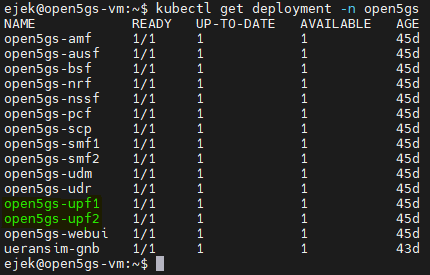
\includegraphics[width=1\linewidth]{53-depy.png}
    \caption{Wdrożenia Open5GS, w tym instancje UPF}\label{fig:53-depy}
\end{figure}

Każdy \textit{pod} w klastrze Kubernetes posiada zdefiniowane wartości dotyczące przydziału zasobów:

\begin{itemize}
    \item \textbf{\texttt{requests}} – określa ilość zasobów CPU oraz pamięci operacyjnej (RAM), jaką dany pod żąda od środowiska chmurowego. Kubernetes zapewnia, że węzeł posiada wystarczające zasoby, aby spełnić te wymagania przed przydzieleniem poda do \textit{węzła}.
    \item \textbf{\texttt{limits}} – maksymalna ilość zasobów, jaką pod może zużyć. Przekroczenie tych wartości skutkuje zakończeniem procesu (np. jego ubiciem w celu ochrony środowiska).
\end{itemize}

Dodatkowo możliwe jest monitorowanie rzeczywistego (aktualnego, chwilowego) wykorzystania procesora i pamięci operacyjnej.

\textbf{Mechanizmy dostępne w Kubernetes}

Kubernetes umożliwia:
\begin{itemize}
    \item monitorowanie bieżącego zużycia CPU oraz pamięci dla konkretnego poda,
    \item monitorowanie zdefiniowanych wartości \texttt{requests} i \texttt{limits} dla konkretnego poda,
    \item aktualizację wartości \texttt{requests} i \texttt{limits} dla konkretnego poda.
\end{itemize}

Wdrożenie komponentu UPF w repozytorium \href{https://github.com/niloysh/open5gs-k8s}{open5gs-k8s} wykorzystuje następujące wartości zasobów:

\begin{lstlisting}[language=sh, caption=Konfiguracja zasobów dla UPF w Open5GS]
resources:
  requests:
    memory: "256Mi"
    cpu: "200m"
  limits:
    memory: "512Mi"
    cpu: "500m"
\end{lstlisting}

Niniejsza konfiguracja jest traktowana jako \textbf{punkt operacyjny}, który powinien być wystarczający w normalnych warunkach (np. przez 80\% czasu). Jednak w sytuacjach, gdy pojedynczy pod UPF sporadycznie przekracza te wartości, konieczne jest zwiększenie dostępnych zasobów oraz proporcjonalne podniesienie limitów.

Zakłada się, że każdorazowe przekroczenie wartości operacyjnych CPU lub pamięci skutkuje przydzieleniem dodatkowych 20\% zasobów dla \texttt{requests} oraz ustawieniem \texttt{limits} na poziomie dwukrotności nowej wartości \texttt{requests}.

\textbf{Przykładowa adaptacja zasobów}

\begin{itemize}
    \item Gdy zużycie CPU osiąga wartość \texttt{270m}:
    \begin{itemize}
        \item \texttt{requests} zostaje zwiększone do \( 270m \times 1.2 = 324m \),
        \item \texttt{limits} zostaje zwiększone do \( 324m \times 2 = 648m \).
    \end{itemize}
    \item Analogiczne zasady dotyczą przydziału pamięci operacyjnej.
\end{itemize}

Jeśli rzeczywiste wykorzystanie zasobów jest znacząco niższe od wartości operacyjnej, nie jest podejmowana żadna akcja korygująca. Nadmierne skalowanie w dół skutkowałoby zbyt częstymi restartami podów, co w konsekwencji generowałoby większe koszty niż wynikające z niedostatecznego wykorzystania zasobów.